\subsubsection{Module MD-10: Quản lý Hệ thống \& Người 
dùng}
Module Quản lý Hệ thống \& Người dùng (MD-10) đóng vai trò là hạt nhân quản trị và cấu hình của toàn bộ hệ thống nhà hàng. Module này cung cấp các công cụ thiết yếu cho Quản trị viên hệ thống và Quản lý nhà hàng để quản lý tài khoản người dùng (nhân viên và khách hàng), phân quyền truy cập, thiết lập các thông số hoạt động chung của nhà hàng, cấu hình các tích hợp với dịch vụ của bên thứ ba (như cổng thanh toán, dịch vụ bot call, dịch vụ giao hàng), và theo dõi hoạt động hệ thống. Sự ổn định, bảo mật và khả năng tùy biến của module này là nền tảng cho hoạt động hiệu quả của tất cả các module nghiệp vụ khác.


\begin{figure}[H]
    \centering
    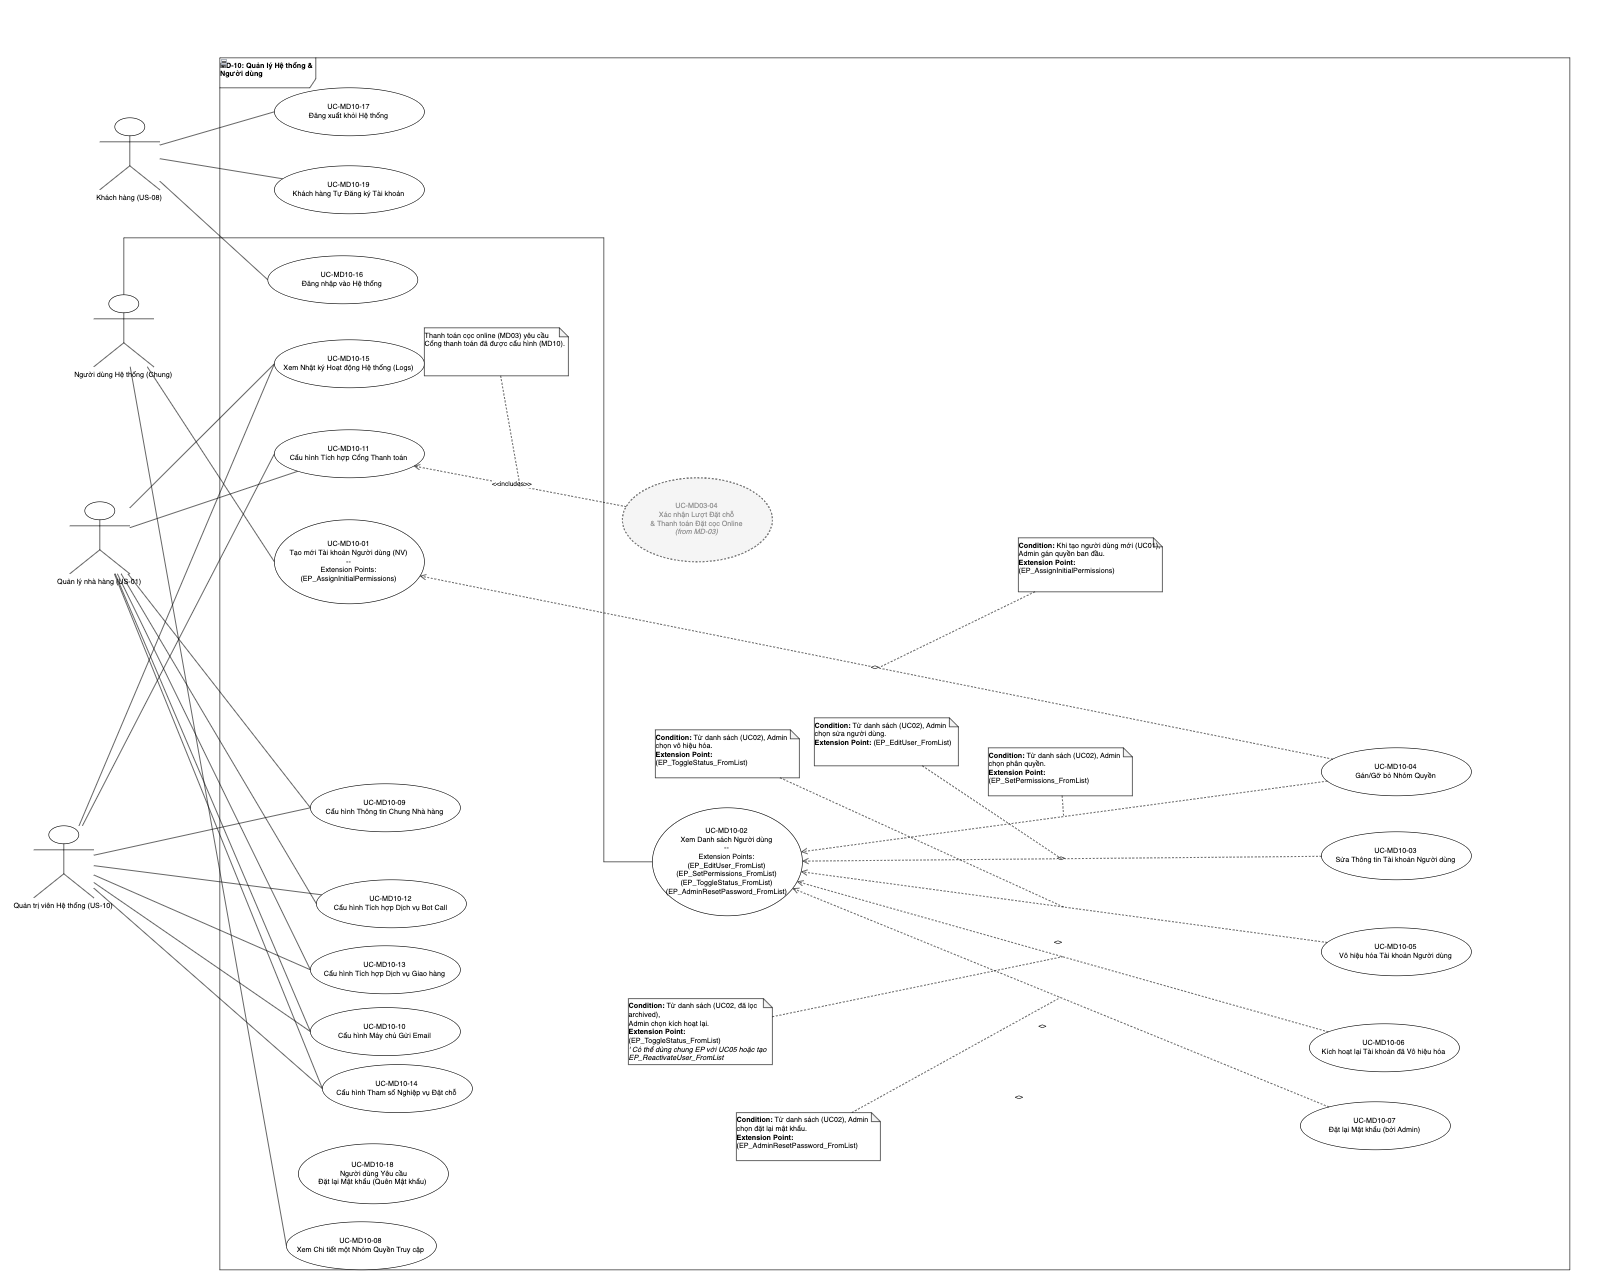
\includegraphics[width=15cm]{Sections/tong_quan/functional_spec/img/uc10.png}
    \vspace{0.5cm}
    \caption{Use case diagram cho Module MD-10}
    \label{fig:my_label}
\end{figure}

\begin{longtable}{|m{2cm}|m{2.5cm}|m{2.5cm}|m{4.5cm}|m{4cm}|}
\caption{Danh sách Yêu cầu Chức năng cho Module MD-10: Quản lý Hệ thống, Người dùng \& Xác thực} 
\hline
\textbf{Mã Module} & \textbf{Mã Yêu cầu CN} & \textbf{Mã Người dùng} & \textbf{Tên Chức năng} & \textbf{Mô tả Ngắn} \
\hline
\endhead % Header cho các trang tiếp theo
\midrule
\endfoot % Footer cho bảng
\bottomrule
\endlastfoot % Footer cho trang cuối cùng
MD-10 & FR-MD10-01 & US-10 & Tạo mới Tài khoản Người dùng (Nhân viên) & Quản trị viên tạo tài khoản đăng nhập mới cho nhân viên, bao gồm thông tin cơ bản. \
\hline
MD-10 & FR-MD10-02 & US-10 & Xem Danh sách Người dùng & Quản trị viên xem danh sách các tài khoản người dùng hiện có trong hệ thống. \
\hline
MD-10 & FR-MD10-03 & US-10 & Sửa Thông tin Tài khoản Người dùng & Quản trị viên cập nhật các thông tin cá nhân, liên hệ của một tài khoản người dùng. \
\hline
MD-10 & FR-MD10-04 & US-10 & Gán/Gỡ bỏ Nhóm Quyền cho Người dùng & Quản trị viên thay đổi các nhóm quyền truy cập mà một người dùng thuộc về. \
\hline
MD-10 & FR-MD10-05 & US-10 & Vô hiệu hóa Tài khoản Người dùng & Quản trị viên tạm khóa (archive) khả năng đăng nhập của một tài khoản người dùng. \
\hline
MD-10 & FR-MD10-06 & US-10 & Kích hoạt lại Tài khoản Người dùng đã Vô hiệu hóa & Quản trị viên mở lại (unarchive) khả năng đăng nhập cho một tài khoản đã bị khóa. \
\hline
MD-10 & FR-MD10-07 & US-10 & Đặt lại Mật khẩu cho Người dùng (bởi Admin) & Quản trị viên hỗ trợ đặt lại mật khẩu cho người dùng (gửi link hoặc đặt trực tiếp). \
\hline
MD-10 & FR-MD10-08 & US-10 & Xem Chi tiết một Nhóm Quyền Truy cập & Quản trị viên xem chi tiết cấu hình và các quyền hạn của một nhóm quyền cụ thể. \
\hline
MD-10 & FR-MD10-09 & US-10, US-01 & Cấu hình Thông tin Chung của Nhà hàng/Công ty & Quản trị viên/Quản lý thiết lập tên, địa chỉ, logo, tiền tệ mặc định cho nhà hàng/công ty. \
\hline
MD-10 & FR-MD10-10 & US-10, US-01 & Cấu hình Máy chủ Gửi Email (Outgoing Email Server) & Quản trị viên/Quản lý thiết lập thông tin máy chủ SMTP để hệ thống có thể gửi email đi. \
\hline
MD-10 & FR-MD10-11 & US-10, US-01 & Cấu hình Tích hợp Cổng Thanh toán & Quản trị viên/Quản lý nhập API keys và các tham số cho các cổng thanh toán trực tuyến. \
\hline
MD-10 & FR-MD10-12 & US-10, US-01 & Cấu hình Tích hợp Dịch vụ Bot Call & Quản trị viên/Quản lý nhập API keys và các tham số vận hành cho dịch vụ Bot Call. \
\hline
MD-10 & FR-MD10-13 & US-10, US-01 & Cấu hình Tích hợp Dịch vụ Giao hàng (Shipday) & Quản trị viên/Quản lý nhập API keys và các tham số vận hành cho dịch vụ Shipday. \
\hline
MD-10 & FR-MD10-14 & US-10, US-01 & Cấu hình Tham số Nghiệp vụ Đặc thù cho Đặt chỗ & Quản trị viên/Quản lý thiết lập các quy tắc kinh doanh như tỷ lệ đặt cọc, giá trị bàn, số ngày gọi bot... \
\hline
MD-10 & FR-MD10-15 & US-10 & Xem Nhật ký Hoạt động Hệ thống (Logs) & Quản trị viên xem các bản ghi log hệ thống để theo dõi, chẩn đoán lỗi và hoạt động. \
\hline
MD-10 & FR-MD10-16 & US-01, US-02, US-03, US-04, US-05, US-06, US-07, US-09, US-10 & Đăng nhập vào Hệ thống & Người dùng cung cấp thông tin xác thực (email/mật khẩu) để truy cập hệ thống. \
\hline
MD-10 & FR-MD10-17 & US-01, US-02, US-03, US-04, US-05, US-06, US-07, US-09, US-10 & Đăng xuất khỏi Hệ thống & Người dùng kết thúc phiên làm việc hiện tại và thoát khỏi hệ thống an toàn. \
\hline
MD-10 & FR-MD10-18 & US-01, US-02, US-03, US-04, US-05, US-06, US-07, US-09, US-10 & Người dùng Yêu cầu Đặt lại Mật khẩu (Quên Mật khẩu) & Người dùng tự yêu cầu hệ thống gửi hướng dẫn đặt lại mật khẩu qua email khi họ quên mật khẩu. \
\hline
MD-10 & FR-MD10-19 & US-08 & Khách hàng Tự Đăng ký Tài khoản & Khách hàng tự tạo tài khoản người dùng trên giao diện web/app để đặt chỗ, quản lý thông tin. \
\hline
\end{longtable}
    

% Bỏ comment và sửa đường dẫn nếu bạn có file ảnh uc10.png
% \begin{figure}[H]
%     \centering
%     % 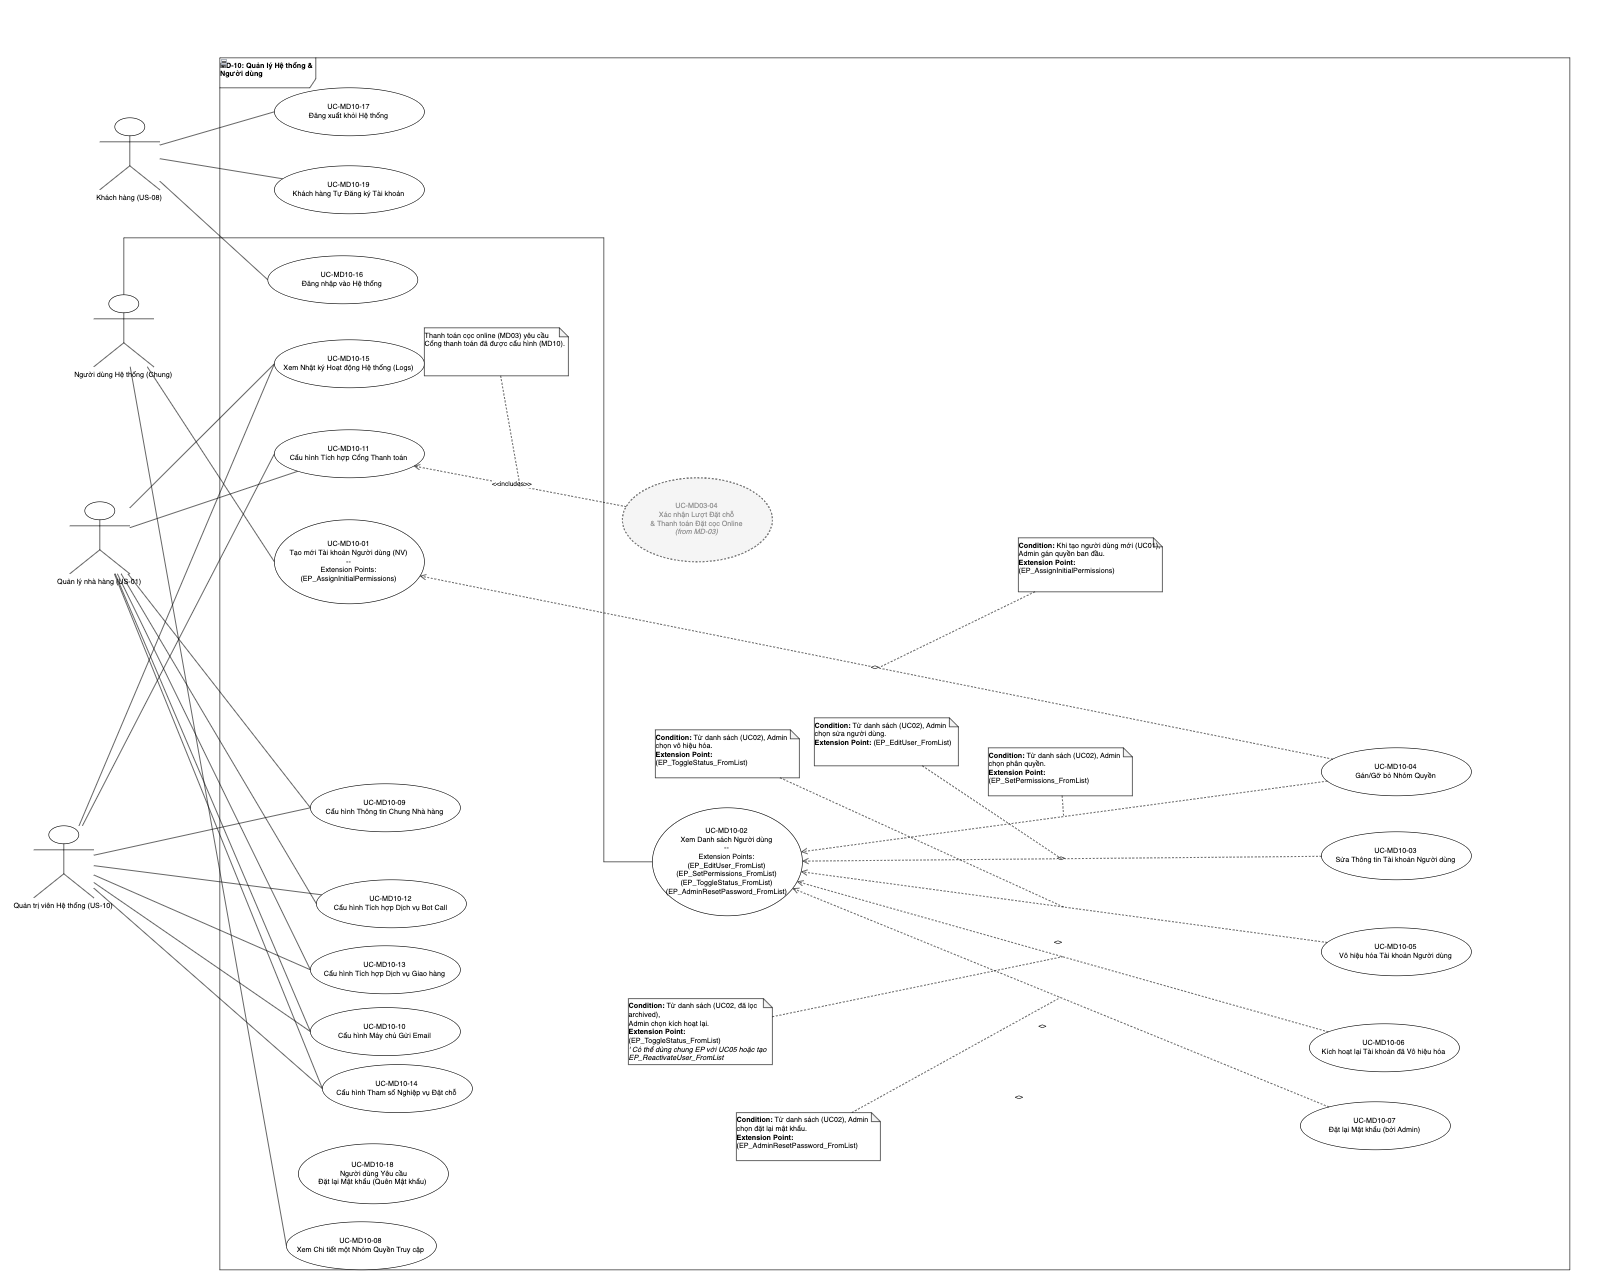
\includegraphics[width=15cm]{Sections/tong_quan/functional_spec/img/uc10.png.png} % Thay thế bằng đường dẫn thực tế đến file ảnh của bạn
%     \caption{Sơ đồ Use Case cho Module MD-10 (Ví dụ)} % Sửa caption nếu cần
%     \label{fig:uc_diagram_md10_full} % Sửa label nếu cần
% \end{figure}

\subsubsubsection{Mục tiêu và Phạm vi}
\label{sssec:md10_objectives_scope_full}
Mục tiêu chính của module MD-10 là:
\begin{itemize}
    \item \textbf{Quản lý tài khoản người dùng toàn diện:} Cho phép tạo, sửa đổi, vô hiệu hóa, kích hoạt lại và quản lý mật khẩu cho tất cả các loại tài khoản người dùng (nhân viên và khách hàng).
    \item \textbf{Kiểm soát truy cập chặt chẽ:} Thông qua việc quản lý các nhóm quyền và gán người dùng vào các nhóm phù hợp, đảm bảo nguyên tắc phân quyền tối thiểu và bảo mật dữ liệu.
    \item \textbf{Cấu hình thông tin và hoạt động chung của nhà hàng:} Thiết lập các thông tin định danh của nhà hàng (tên, địa chỉ, logo), đơn vị tiền tệ, và các tham số nghiệp vụ đặc thù ảnh hưởng đến hoạt động của các module khác (ví dụ: quy tắc đặt cọc cho module đặt chỗ).
    \item \textbf{Quản lý tích hợp với các dịch vụ bên thứ ba:} Cho phép cấu hình và quản lý kết nối API với các dịch vụ thiết yếu như máy chủ gửi email, cổng thanh toán trực tuyến, dịch vụ bot call, và dịch vụ quản lý giao hàng.
    \item \textbf{Cung cấp cơ chế xác thực an toàn:} Đảm bảo quy trình đăng nhập, đăng xuất và đặt lại mật khẩu được thực hiện một cách an toàn và hiệu quả.
    \item \textbf{Theo dõi và chẩn đoán hệ thống:} Cung cấp khả năng xem nhật ký hoạt động của hệ thống để hỗ trợ việc giám sát, chẩn đoán và khắc phục sự cố.
\end{itemize}
Phạm vi của module bao gồm toàn bộ vòng đời quản lý người dùng, quản lý phân quyền, cấu hình các thông số hệ thống cơ bản và các tích hợp quan trọng, cũng như các chức năng xác thực người dùng và theo dõi log hệ thống.

\subsubsubsection{Đối tượng Sử dụng Chính}
\label{sssec:md10_primary_users_full}
Module này phục vụ nhiều nhóm đối tượng người dùng với các vai trò khác nhau:
\begin{itemize}
    \item \textbf{US-10 (Quản trị viên Hệ thống):} Là người dùng có quyền hạn cao nhất, chịu trách nhiệm chính trong việc tạo và quản lý tài khoản người dùng (nhân viên), phân quyền, cấu hình các tích hợp kỹ thuật (máy chủ email, API), và xem log hệ thống.
    \item \textbf{US-01 (Quản lý nhà hàng):} Có thể được cấp quyền để cấu hình một số thông tin chung của nhà hàng, các tham số nghiệp vụ, và một số tích hợp dịch vụ (cổng thanh toán, bot call, giao hàng). Cũng có thể có quyền quản lý một số khía cạnh của tài khoản nhân viên.
    \item \textbf{US-01, US-02, US-03, US-04, US-05, US-06, US-07, US-09 (Tất cả Nhân viên có tài khoản):} Là người dùng của các chức năng xác thực cơ bản như Đăng nhập, Đăng xuất, và Yêu cầu Đặt lại Mật khẩu khi quên.
    \item \textbf{US-08 (Khách hàng):} Là người dùng của chức năng Tự Đăng ký Tài khoản trên giao diện web/app của nhà hàng.
\end{itemize}

\subsubsubsection{Các Chức năng Chính}
\label{sssec:md10_key_functionalities_full}
Module MD-10 cung cấp một bộ các chức năng quản trị và cấu hình hệ thống toàn diện, được mô tả chi tiết qua các Use Case sau:

\begin{itemize}
    \item \textbf{Quản lý Tài khoản Người dùng (Nhân viên) (UC-MD10-01 đến UC-MD10-07):}
    \begin{itemize}
        \item Tạo mới tài khoản đăng nhập cho nhân viên (UC-MD10-01).
        \item Xem danh sách tất cả các tài khoản người dùng trong hệ thống (UC-MD10-02).
        \item Sửa đổi thông tin cá nhân và liên hệ của một tài khoản người dùng (UC-MD10-03).
        \item Gán hoặc gỡ bỏ các Nhóm Quyền truy cập cho một người dùng để xác định phạm vi hoạt động (UC-MD10-04).
        \item Vô hiệu hóa (tạm khóa) khả năng đăng nhập của một tài khoản người dùng (UC-MD10-05).
        \item Kích hoạt lại một tài khoản người dùng đã bị vô hiệu hóa trước đó (UC-MD10-06).
        \item Quản trị viên hỗ trợ đặt lại mật khẩu cho một người dùng (UC-MD10-07).
    \end{itemize}

    \item \textbf{Quản lý Phân quyền (UC-MD10-08):}
    \begin{itemize}
        \item Xem chi tiết cấu hình và các quyền hạn cụ thể của một Nhóm Quyền truy cập đã tồn tại (UC-MD10-08).
    \end{itemize}

    \item \textbf{Cấu hình Hệ thống và Tích hợp (UC-MD10-09 đến UC-MD10-14):}
    \begin{itemize}
        \item Thiết lập các thông tin chung của nhà hàng/công ty như tên, địa chỉ, logo, tiền tệ (UC-MD10-09).
        \item Cấu hình thông tin máy chủ SMTP để hệ thống có thể gửi email (UC-MD10-10).
        \item Nhập API keys và các tham số để tích hợp với các cổng thanh toán trực tuyến (UC-MD10-11).
        \item Nhập API keys và các tham số vận hành để tích hợp với dịch vụ Bot Call (UC-MD10-12, liên quan FR-MD04-05).
        \item Nhập API keys và các tham số vận hành để tích hợp với dịch vụ quản lý giao hàng Shipday (UC-MD10-13, liên quan FR-MD07-15).
        \item Thiết lập các quy tắc và tham số nghiệp vụ đặc thù cho chức năng Đặt chỗ (ví dụ: tỷ lệ đặt cọc, giá trị bàn, số ngày gọi bot) (UC-MD10-14, liên quan FR-MD03-15 và FR-MD04-05).
    \end{itemize}

    \item \textbf{Theo dõi và Bảo trì Hệ thống (UC-MD10-15):}
    \begin{itemize}
        \item Cho phép Quản trị viên xem các bản ghi nhật ký hoạt động của hệ thống để theo dõi và chẩn đoán lỗi (UC-MD10-15).
    \end{itemize}

    \item \textbf{Xác thực Người dùng (UC-MD10-16 đến UC-MD10-19):}
    \begin{itemize}
        \item Cho phép tất cả người dùng có tài khoản (nhân viên, khách hàng) đăng nhập vào hệ thống bằng tên đăng nhập/email và mật khẩu (UC-MD10-16).
        \item Cho phép người dùng đã đăng nhập kết thúc phiên làm việc và thoát khỏi hệ thống một cách an toàn (UC-MD10-17).
        \item Cho phép người dùng tự yêu cầu hệ thống gửi hướng dẫn đặt lại mật khẩu qua email khi họ quên mật khẩu (UC-MD10-18).
        \item Cho phép khách hàng mới tự tạo tài khoản người dùng trên giao diện web/app của nhà hàng (UC-MD10-19).
    \end{itemize}
\end{itemize}

\subsubsubsection{Tóm tắt Luồng Hoạt động Tổng thể}
\label{sssec:md10_overall_workflow_full}
Luồng hoạt động trong module MD-10 rất đa dạng, phụ thuộc vào vai trò của người dùng và nhu cầu cụ thể. Một số luồng chính bao gồm:
\begin{enumerate}
    \item \textbf{Thiết lập hệ thống ban đầu hoặc khi có thay đổi lớn:}
        \begin{itemize}
            \item Quản trị viên/Quản lý Cấu hình Thông tin Chung của Nhà hàng (UC-MD10-09).
            \item Cấu hình Máy chủ Gửi Email (UC-MD10-10).
            \item Cấu hình Tích hợp Cổng Thanh toán (UC-MD10-11).
            \item Cấu hình Tích hợp Dịch vụ Bot Call (UC-MD10-12).
            \item Cấu hình Tích hợp Dịch vụ Giao hàng (Shipday) (UC-MD10-13).
            \item Cấu hình Tham số Nghiệp vụ Đặc thù cho Đặt chỗ (UC-MD10-14).
        \end{itemize}
    \item \textbf{Quản lý tài khoản nhân viên:}
        \begin{itemize}
            \item Quản trị viên Tạo mới Tài khoản Người dùng (Nhân viên) (UC-MD10-01).
            \item Gán/Gỡ bỏ Nhóm Quyền cho Người dùng (UC-MD10-04) (có thể tham khảo UC-MD10-08 để hiểu rõ nhóm quyền).
            \item Khi cần, Sửa Thông tin Tài khoản Người dùng (UC-MD10-03).
            \item Hỗ trợ Đặt lại Mật khẩu cho Người dùng (bởi Admin) (UC-MD10-07) nếu nhân viên yêu cầu.
            \item Vô hiệu hóa Tài khoản Người dùng (UC-MD10-05) khi nhân viên nghỉ việc, hoặc Kích hoạt lại Tài khoản Người dùng đã Vô hiệu hóa (UC-MD10-06) khi cần.
            \item Quản trị viên thường xuyên Xem Danh sách Người dùng (UC-MD10-02) để kiểm tra.
        \end{itemize}
    \item \textbf{Quy trình xác thực của tất cả người dùng:}
        \begin{itemize}
            \item Người dùng (nhân viên hoặc khách hàng đã đăng ký) Đăng nhập vào Hệ thống (UC-MD10-16).
            \item Nếu quên mật khẩu, người dùng Yêu cầu Đặt lại Mật khẩu (Quên Mật khẩu) (UC-MD10-18).
            \item Sau khi làm việc xong, người dùng Đăng xuất khỏi Hệ thống (UC-MD10-17).
        \end{itemize}
    \item \textbf{Khách hàng tự đăng ký (nếu có kênh online):}
        \begin{itemize}
            \item Khách hàng mới Tự Đăng ký Tài khoản (UC-MD10-19) trên website/app.
        \end{itemize}
    \item \textbf{Theo dõi và bảo trì hệ thống:}
        \begin{itemize}
            \item Quản trị viên Xem Nhật ký Hoạt động Hệ thống (Logs) (UC-MD10-15) để chẩn đoán sự cố hoặc theo dõi hoạt động.
        \end{itemize}
\end{enumerate}
Module MD-10 là xương sống đảm bảo cho toàn bộ hệ thống nhà hàng có thể vận hành một cách trơn tru, an toàn và tuân thủ các quy định, chính sách đã đặt ra.

